% How maxent_upgrade works: the two inputs, the solve, the outputs.
% Drawn at its printed size (15 cm wide, every label at 10-11 pt), so it can be
% included at \textwidth in the JHEP paper and used as the README image.
%
% Build (from this directory):
%   pdflatex flowchart.tex
%   pdftocairo -svg flowchart.pdf flowchart.svg
%   pdftoppm -png -singlefile -scale-to-x 1600 -scale-to-y -1 flowchart.pdf flowchart
%
% Every box names what the code does:
%   NNLOJET + patch     nnlojet_patch/ (event-level accumulators of T_n, per order, per run)
%   export_moments.py   pools the runs (ratio of summed accumulators; stat. = run scatter,
%                       scale = 7-point half-range; window rates)
%   moments/*.json      the released tables;  maxent_upgrade.load_moments(process)
%   upgrade()           maxent_upgrade/__init__.py: umap/cheb, profile_w, resolved_order,
%                       _newton_maxent (z-scored, damped Newton on the dual, ridge L2)
%   bands               re-solves with config['lam0'] = result.report['lam'] and
%                       fixed_orders = the central chosen orders (eventlevel/make_dy_band_weights.py),
%                       from the released per-run accumulators (scale variants, bootstrap of the runs)
\documentclass[11pt,tikz,border=0pt]{standalone}
\usepackage[T1]{fontenc}
\usepackage{lmodern}
\usepackage{amsmath}
\usepackage{microtype}
\usetikzlibrary{arrows.meta,calc,backgrounds}
\pgfdeclarelayer{canvas}
\pgfsetlayers{canvas,background,main}

% palette: the MaxEnt red of the paper's figures is the one accent; inputs and
% outputs are a cool grey (fixed order), a warm grey (prior) and a neutral grey
\definecolor{ink}{HTML}{222222}
\definecolor{soft}{HTML}{4A4A4A}
\definecolor{mx}{HTML}{D62728}
\definecolor{mxbg}{HTML}{FDF3F3}
\definecolor{fo}{HTML}{687789}
\definecolor{fobg}{HTML}{EBF0F5}
\definecolor{pr}{HTML}{978874}
\definecolor{prbg}{HTML}{F5F0EA}
\definecolor{out}{HTML}{8F8F8F}
\definecolor{outbg}{HTML}{F2F2F2}
\definecolor{arr}{HTML}{5A5A5A}

\newcommand{\lane}[1]{\textls[160]{\textsc{#1}}}
\newcommand{\ttt}[1]{\texttt{#1}}
\newcommand{\sft}[1]{{\color{soft}#1}}

\begin{document}
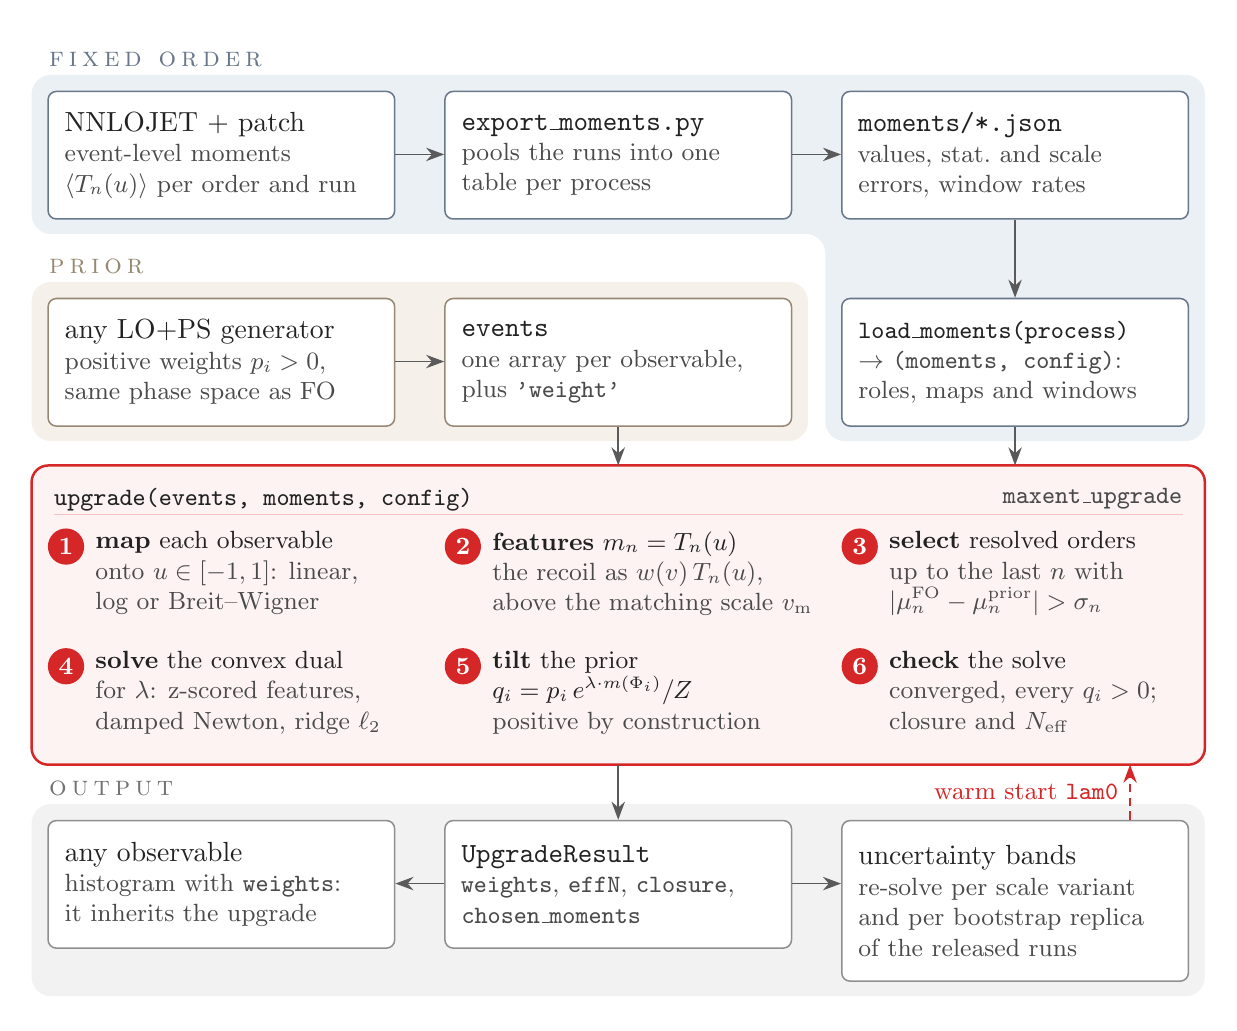
\begin{tikzpicture}[
  font=\small, text=ink,
  box/.style={rounded corners=3pt, line width=0.55pt, inner xsep=6pt, inner ysep=4.5pt,
              align=flush left, text width=3.98cm, minimum height=1.62cm, anchor=north},
  fobx/.style={box, draw=fo, fill=white},
  prbx/.style={box, draw=pr, fill=white},
  outbx/.style={box, draw=out, fill=white},
  cell/.style={align=flush left, text width=#1, inner sep=0pt, anchor=north west},
  cell/.default=4.0cm,
  badge/.style={circle, fill=mx, text=white, inner sep=0pt, minimum size=4.6mm, font=\small\bfseries},
  flow/.style={-{Stealth[length=2.3mm,width=1.7mm]}, line width=0.6pt, draw=arr},
]
% three columns of 4.42 cm boxes, x = [0.25,4.67], [5.29,9.71], [10.33,14.75]
\def\ca{2.46}\def\cb{7.5}\def\cc{12.54}
\def\la{0.25}\def\lb{5.29}\def\lc{10.33}\def\rc{14.75}\def\bw{4.42}
\def\yA{10.75}   % top of row 1 (fixed order)
\def\yB{8.12}    % top of row 2 (prior, and load)
\def\yC{5.99}    % top of the core
\def\hC{3.8}     % height of the core
\def\yD{1.49}    % top of the outputs
\def\hB{1.62}    % box height
\def\ym{0.81}    % horizontal arrows run at mid-height of a box
\def\pad{0.2}    % lane padding

% ---------------- fixed-order lane ----------------
\node[fobx] (nj) at (\ca,\yA) {{\normalsize NNLOJET + patch}\\
  \sft{event-level moments\\ $\langle T_n(u)\rangle$ per order and run}};
\node[fobx] (ex) at (\cb,\yA) {{\normalsize\ttt{export\_moments.py}}\\
  \sft{pools the runs into one\\ table per process}};
\node[fobx] (js) at (\cc,\yA) {{\normalsize\ttt{moments/*.json}}\\
  \sft{values, stat.\ and scale\\ errors, window rates}};
\node[fobx] (ld) at (\cc,\yB) {{\ttt{load\_moments(process)}}\\
  \sft{$\to$ \ttt{(moments, config)}:\\ roles, maps and windows}};
\draw[flow] (\la+\bw,\yA-\ym) -- (\lb,\yA-\ym);
\draw[flow] (\lb+\bw,\yA-\ym) -- (\lc,\yA-\ym);
\draw[flow] (js) -- (ld);

% ---------------- prior lane ----------------
\node[prbx] (gen) at (\ca,\yB) {{\normalsize any LO+PS generator}\\
  \sft{positive weights $p_i>0$,\\ same phase space as FO}};
\node[prbx] (ev) at (\cb,\yB) {{\normalsize\ttt{events}}\\
  \sft{one array per observable,\\ plus \ttt{'weight'}}};
\draw[flow] (\la+\bw,\yB-\ym) -- (\lb,\yB-\ym);

% ---------------- the solve ----------------
\node[anchor=north west, inner sep=0pt] at (\la+0.08,\yC-0.28) {\ttt{upgrade(events, moments, config)}};
\node[anchor=north east, inner sep=0pt, text=soft] at (\rc-0.08,\yC-0.28) {\ttt{maxent\_upgrade}};
\foreach \k/\x in {1/\la, 2/\lb, 3/\lc} { \node[badge, anchor=west] (b\k) at (\x,\yC-1.03) {\k}; }
\foreach \k/\x in {4/\la, 5/\lb, 6/\lc} { \node[badge, anchor=west] (b\k) at (\x,\yC-2.55) {\k}; }
\node[cell] at ($(b1.east)+(0.13,0.2)$) {\textbf{map} each observable\\
  \sft{onto $u\in[-1,1]$: linear,\\ log or Breit--Wigner}};
\node[cell=4.3cm] at ($(b2.east)+(0.13,0.2)$) {\textbf{features} $m_n=T_n(u)$\\
  \sft{the recoil as $w(v)\,T_n(u)$,\\ above the matching scale $v_\mathrm{m}$}};
\node[cell=3.85cm] at ($(b3.east)+(0.13,0.2)$) {\textbf{select} resolved orders\\
  \sft{up to the last $n$ with\\ $|\mu_n^{\mathrm{FO}}-\mu_n^{\mathrm{prior}}|>\sigma_n$}};
\node[cell] at ($(b4.east)+(0.13,0.2)$) {\textbf{solve} the convex dual\\
  \sft{for $\lambda$: z-scored features,\\ damped Newton, ridge $\ell_2$}};
\node[cell] at ($(b5.east)+(0.13,0.2)$) {\textbf{tilt} the prior\\
  $q_i=p_i\,e^{\lambda\cdot m(\Phi_i)}/Z$\\ \sft{positive by construction}};
\node[cell=3.85cm] at ($(b6.east)+(0.13,0.2)$) {\textbf{check} the solve\\
  \sft{converged, every $q_i>0$;\\ closure and $N_\mathrm{eff}$}};
\begin{scope}[on background layer]
  \draw[draw=mx, line width=0.9pt, fill=mxbg, rounded corners=6pt] (0.05,\yC) rectangle (14.95,\yC-\hC);
  \draw[mx!28, line width=0.5pt] (\la+0.08,\yC-0.62) -- (\rc-0.08,\yC-0.62);
\end{scope}
\draw[flow] (ev) -- (\cb,\yC);
\draw[flow] (ld) -- (\cc,\yC);

% ---------------- outputs ----------------
\node[outbx] (fol) at (\ca,\yD) {{\normalsize any observable}\\
  \sft{histogram with \ttt{weights}:\\ it inherits the upgrade}};
\node[outbx] (res) at (\cb,\yD) {{\normalsize\ttt{UpgradeResult}}\\
  \sft{\ttt{weights}, \ttt{effN}, \ttt{closure},\\ \ttt{chosen\_moments}}};
\node[outbx, minimum height=2.04cm] (band) at (\cc,\yD) {{\normalsize uncertainty bands}\\
  \sft{re-solve per scale variant\\ and per bootstrap replica\\ of the released runs}};
\draw[flow] (\cb,\yC-\hC) -- (res);
\draw[flow] (\lb,\yD-\ym) -- (\la+\bw,\yD-\ym);
\draw[flow] (\lb+\bw,\yD-\ym) -- (\lc,\yD-\ym);
\draw[-{Stealth[length=2.3mm,width=1.7mm]}, line width=0.6pt, draw=mx, densely dashed]
   (\rc-0.75,\yD) -- (\rc-0.75,\yC-\hC) node[midway, left, text=mx, inner sep=4pt] {warm start \ttt{lam0}};

% ---------------- lanes ----------------
\begin{scope}[on background layer]
  % fixed order: an L along row 1 that turns down into the solve
  \fill[fobg, rounded corners=7pt]
    (\la-\pad,\yA+\pad) -- (\rc+\pad,\yA+\pad) -- (\rc+\pad,\yB-\hB-\pad) -- (\lc-\pad,\yB-\hB-\pad)
    -- (\lc-\pad,\yA-\hB-\pad) -- (\la-\pad,\yA-\hB-\pad) -- cycle;
  \fill[prbg, rounded corners=7pt] (\la-\pad,\yB+\pad) rectangle (\lb+\bw+\pad,\yB-\hB-\pad);
  \fill[outbg, rounded corners=7pt] (\la-\pad,\yD+\pad) rectangle (\rc+\pad,\yD-2.04-\pad);
\end{scope}
\node[anchor=south west, text=fo, inner sep=1pt, font=\normalsize] at (\la-0.05,\yA+\pad+0.07) {\lane{fixed order}};
\node[anchor=south west, text=pr, inner sep=1pt, font=\normalsize] at (\la-0.05,\yB+\pad+0.07) {\lane{prior}};
\node[anchor=south west, text=out!80!black, inner sep=1pt, font=\normalsize] at (\la-0.05,\yD+\pad+0.07) {\lane{output}};

% white ground, so the SVG and PNG read on a dark page too
\begin{pgfonlayer}{canvas}
  \fill[white] (0,\yD-2.04-\pad-0.08) rectangle (15,\yA+\pad+0.6);
\end{pgfonlayer}
\end{tikzpicture}
\end{document}
